%%
%% Framesoc User Guide
%%

\documentclass[twoside]{article}
\usepackage[a4paper]{geometry}
\usepackage[utf8]{inputenc}
\usepackage[T1]{fontenc}
\usepackage{RR}
\usepackage{epsfig}
\usepackage[english]{babel}
\usepackage{cite}
\usepackage{float}
\usepackage{graphicx}
\usepackage{subcaption}
\usepackage{textcomp}
\usepackage[hidelinks]{hyperref} % hide link squares
\usepackage{listings}



%%
%% date
\RRdate{May 2015}
%%
%% If version 2
%% \RRversion{2}
%% version 2 date
%% \RRdater{November 2008}
%%
\RRauthor{
Generoso Pagano\thanks{INRIA, firstname.lastname@inria.fr}, Youenn Corre\footnotemark[1]
}
%% On each even page
\authorhead{Framesoc User Guide}
%% French title
\RRtitle{Framesoc User Guide \LARGE{\numVersion}}
%% English title
\RRetitle{Framesoc User Guide \\\footnotesize{~ } \\ \large{\numVersion}}
%%
\titlehead{Framesoc User Guide}
%%
\RRprojet{MESCAL}
%%
\URRhoneAlpes 
%%
\RCGrenoble 
%%
\abstract{This guide describes the Framesoc workbench, which is the desktop user environment provided by Framesoc infrastructure. The document targets the end-users.}

%%=====================================================================
%%=====================================================================
\begin{document}

\begin{sloppypar} %% avoid long words exceeding margins
%%=====================================================================
%%=====================================================================

\interfootnotelinepenalty=10000 %% allow long footnotes

%%=====================================================================
%% Custom commands
\newcommand{\parag}[1]{\paragraph{#1}\mbox{}\\}
\newcommand{\subparag}[1]{\subparagraph{#1}\mbox{}\\}
\newcommand{\subsubparag}[1]{\subparagraph{#1}}
\newcommand{\num}[1]{\textcolor{red}{#1}}
\newcommand{\numVersion}{v1.0.7}
%% 
%% Itemize
\renewcommand{\labelitemi}{$\bullet$}
\renewcommand{\labelitemii}{$\circ$}
%%=====================================================================

%%
\makeRT 
%%

%%=====================================================================
\renewcommand{\contentsname}{Table of contents}
\tableofcontents
\newpage
%%=====================================================================
%=====================================================================
\section{Introduction}
\label{sec:introduction}

%=====================================================================

Framesoc, the SoC-Trace project~\cite{SoC-TRACE} trace management infrastructure, is composed by three main layers, as shown in Figure~\ref{fig:architecture}.

\begin{figure}[h]
  \centering
    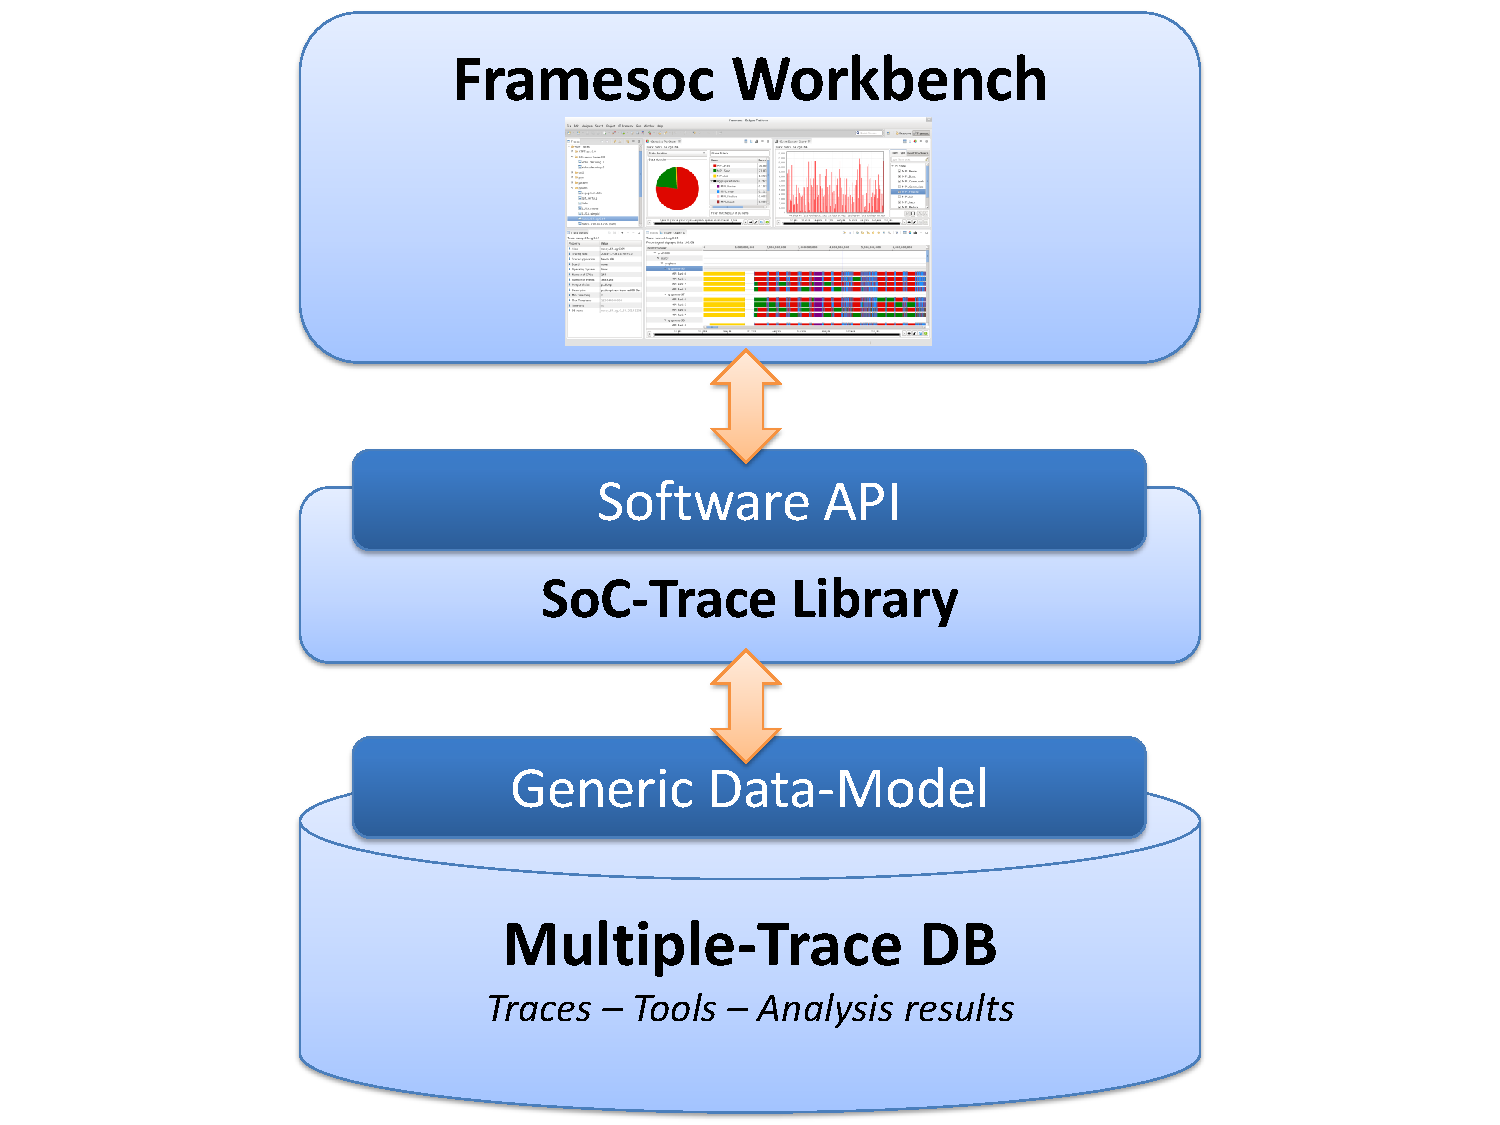
\includegraphics[width=0.7\textwidth]{images/framesoc_architecture.pdf}
  \caption{Framesoc Architecture}
  \label{fig:architecture}
\end{figure}

At the lowest level, there is a Multiple-Trace database, which stores all the data concerning traces, analysis tools and the analysis result produced by thees tools, using a generic data-model.
Above this layer, the SoC-Trace library provides a software API to facilitate the interaction with the data-model and help the implementation of trace tools.
On top of this software library, Framesoc provides a graphical user environment, facilitating trace management, basic trace analysis and tool management.

This guide describes Framesoc from the user perspective (i.e., Framesoc graphical user environment). 
More information about the lowest layers of Framesoc infrastructure can be found in the technical report RT-427~\cite{pagano:hal} and the research report RR-LIG-046~\cite{rrlig46}.

\newpage

%=====================================================================
\section{Installation and Setup}
\label{sec:installation}
%=====================================================================

Framesoc is an application built on top of the Eclipse framework. Therefore, the easiest way to install Framesoc is to use its Eclipse update site, as explained in the online wiki page: \url{https://github.com/soctrace-inria/framesoc/wiki/Install-and-setup-a-standalone-version-of-Framesoc-using-the-update-site}.

%=====================================================================
\section{Framesoc Perspective}
\label{sec:perspective}
%=====================================================================

\begin{figure}[h!]
  \centering
    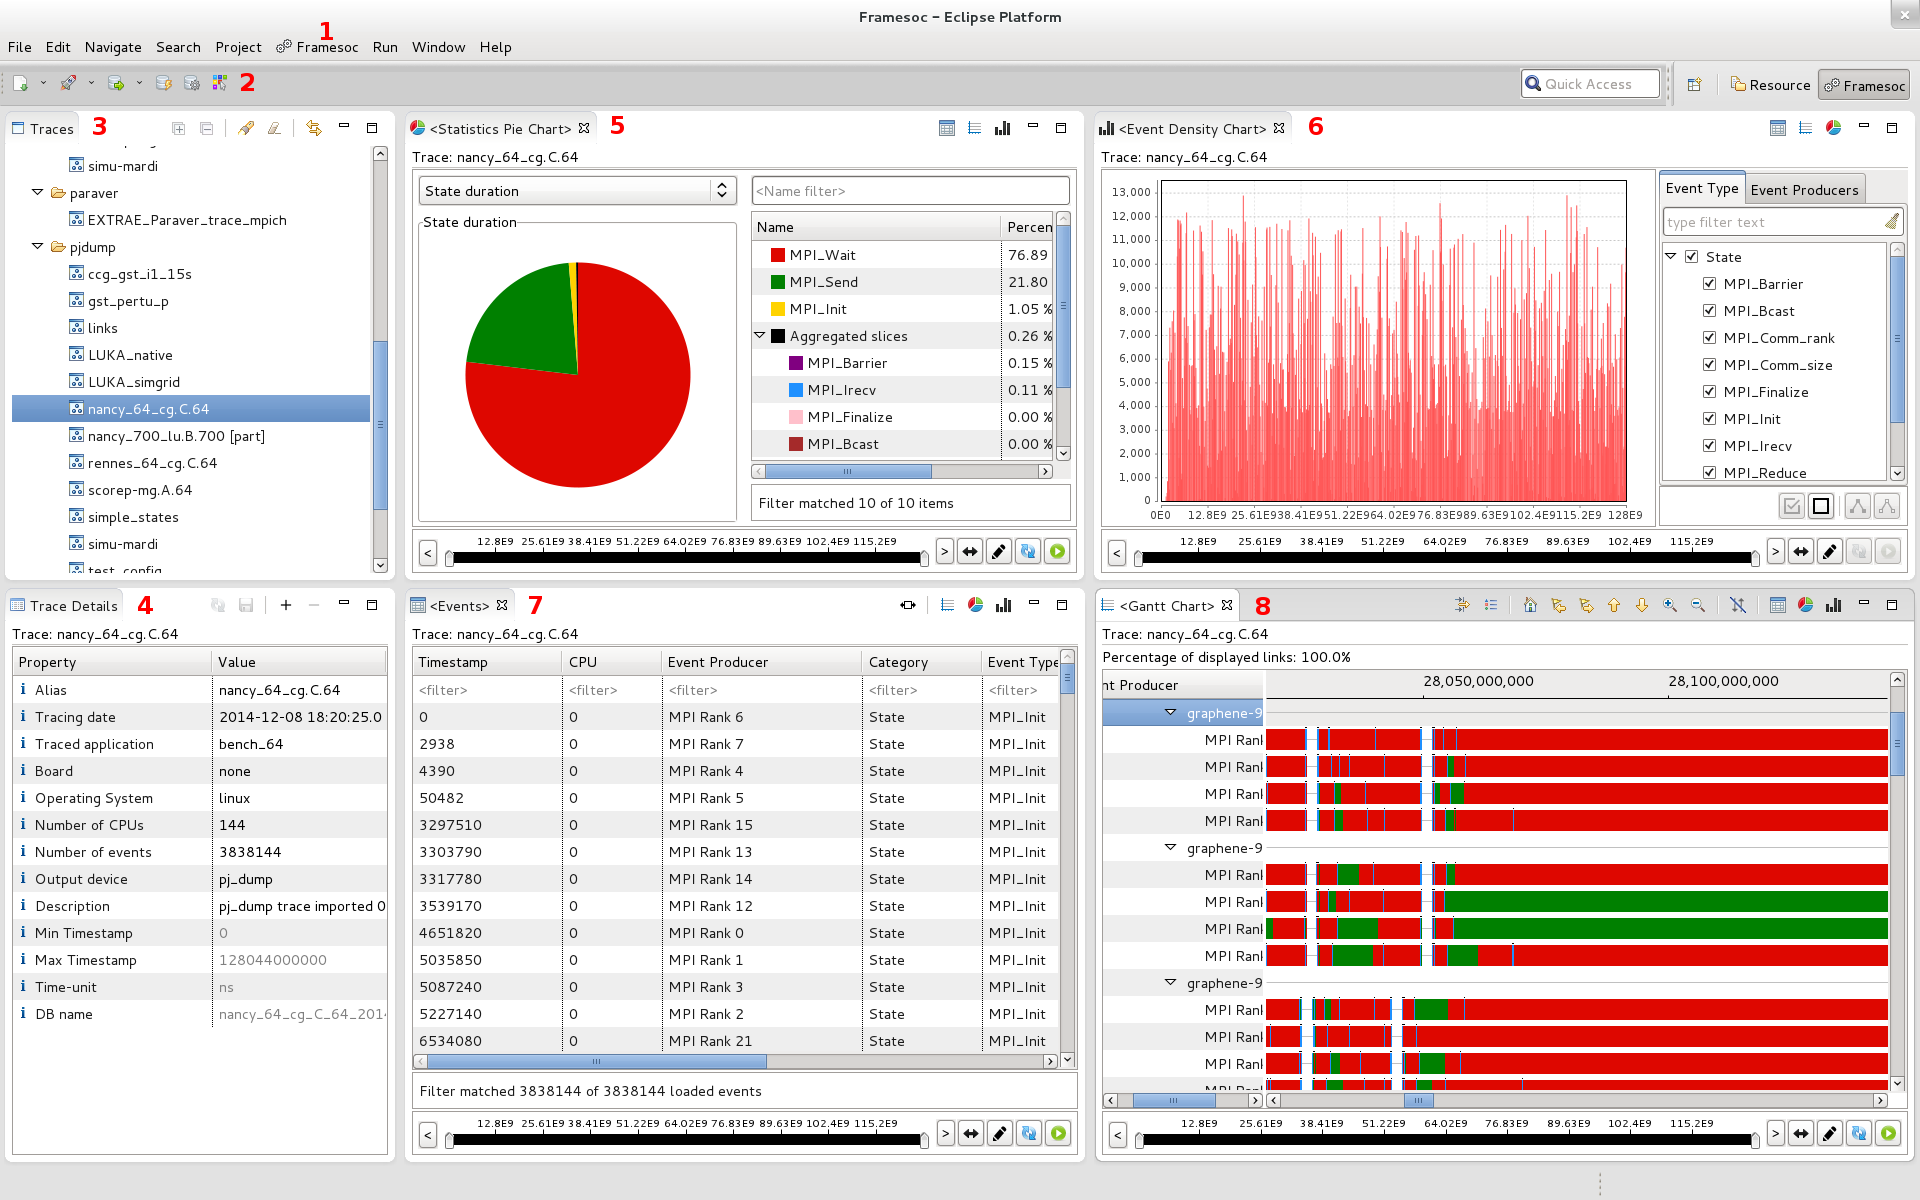
\includegraphics[width=1.0\textwidth]{images/perspective_numbers.png}
  \caption{Framesoc Eclipse Perspective}
  \label{fig:all_perspective}
\end{figure}

Framesoc provides an Eclipse perspective\footnote{Within an Eclipse application, a perspective defines an initial set and layout of views, menu and toolbars. The Framesoc Eclipse perspective can be activated by selecting it from the \textbf{Window $>$ Open Perspective $>$ Other... $>$ Framesoc} menu.} for trace management and analysis.
The Framesoc perspective (Figure~\ref{fig:all_perspective}) contains the following elements:
\begin{itemize}
 \item A Framesoc menu (\num{1}).
 \item A toolbar (\num{2}).
 \item A set of views for trace management and analysis. We find on the left the two \emph{management views}: a trace browser (\num{3}) and a trace metadata viewer/editor (\num{4}). On the right, there are four \emph{analysis views}: a statistics pie chart (\num{5}), an event density chart (\num{6}), an event table (\num{7}), and a Gantt chart (\num{8}). 
\end{itemize}

The management views (trace browser and metadata viewer/editor) refer to the whole system and are typically the entry point for trace analysis.
For this reason, they cannot be closed and there can be only a single instance of each of them.
On the contrary, all the analysis views refer to a single trace, so they can be opened and closed as needed. 
The alias of the trace currently shown within an analysis view is displayed as the view name, beside the view icon.
For each trace, there can be an instance of each type of analysis view. 
The maximum number of open instances for a given type of analysis view is configurable (Appendix~\ref{app:conf}).
When a trace is selected in the trace browser, the corresponding metadata are shown in the metadata viewer and all the analysis views referring to that trace (if any) are highlighted. 
Namely, the view name (which corresponds to the trace alias) is preceded by an arrow (\emph{>}). 
In the example shown in Figure~\ref{fig:all_perspective}, all analysis views refer to the selected trace \texttt{nancy\_64\_cg.C.64}.
On the other hand, when an analysis view is given focus, the trace shown in that view becomes the selected trace in the trace browser, so the metadata viewer is updated accordingly and all the analysis views are consistently highlighted or unhighlighted. 

The following sections describe in detail Framesoc management and analysis views, as well as the functionalities accessible via Framesoc menu and toolbar.

%=====================================================================
\section{Management Views}
\label{sec:management}
%=====================================================================

%------------------------------------------------------------------
\subsection{Trace Browser}
\label{subsec:explorer}

\begin{figure}[h!]
  \centering
    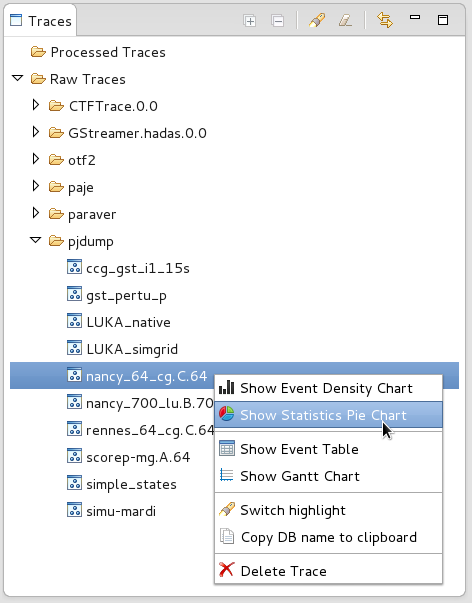
\includegraphics[width=0.5\textwidth]{images/trace_browser_popup.png}
  \caption{Traces view}
  \label{fig:popup_explorer}
\end{figure}

The \emph{Traces} view (Figure~\ref{fig:popup_explorer}) is the Framesoc perspective trace browser.
Traces are presented in a tree viewer with a two-level hierarchy. 
The first level distinguishes processed traces from raw traces~\footnote{As described in the technical report RT-427~\cite{pagano:hal}, a processed trace is a trace created by an analysis tool as the result of an analysis on another trace.}. 
Then, in each of these two categories, traces are grouped by type. 
The type may relate to the trace format or to the tool that created the trace. 
The viewer presents a trace alias for each trace.

Double-clicking on a trace opens the Gantt Chart for that trace (Subsection~\ref{subsec:gantt}).
Right-clicking on a single trace opens a context menu that gives access to the following functionalities:
\begin{itemize}
 \item \emph{Show Event Density Chart}: open the density chart view for this trace (see Subsection~\ref{subsec:histogram}).
 \item \emph{Show Statistics Pie Chart}: open the pie chart view for this trace (see Subsection~\ref{subsec:pie}).
 \item \emph{Show Event Table}: open the event table view for this trace (see Subsection~\ref{subsec:table}).
 \item \emph{Show Gantt Chart}: open the Gantt chart view for this trace (see Subsection~\ref{subsec:gantt}).
 \item \emph{Switch highlight}: switch the highlight state of the trace in the browser (see Figure~\ref{fig:highlight}). A trace being highlighted in the browser is shown in bold.
 \item \emph{Copy DB name to clipboard}: copy to the clipboard the name of the database containing the trace raw data.
 \item \emph{Delete Trace}: delete the trace from the system.
\end{itemize}
Extra options in this menu may be available, depending on the tools currently installed in Framesoc. For instance, if Ocelotl is installed, then a new line is added to open the trace with Ocelotl (i.e. \emph{Show Ocelotl}).
If more than one trace is selected, only the \emph{Switch highlight} and \emph{Delete Trace} entries are displayed in this context menu.
Note that if one or more traces are deleted, an update notification is sent to the other views.
This allows a view to do the necessary actions if the trace it displays has been deleted.

The view toolbar contains the following buttons: a couple of buttons to expand (\num{1}) and collapse (\num{2}) the trace hierarchy, a button to launch the \emph{Trace Filter Dialog} (\num{3}, see Subsection~\ref{subsubsec:trace_filter}), a button to clean the highlight state of all traces (\num{4}, see Subsection~\ref{subsubsec:trace_filter}) and a button to manually resynchronize the displayed traces with the information contained in the Framesoc System DB\footnote{See the technical report RT-427~\cite{pagano:hal} for further details on the database architecture.} (\num{5}).

\subsubsection{Trace Filter}
\label{subsubsec:trace_filter}

Pressing the button indicated as \num{3} in Figure~\ref{fig:popup_explorer}, the \emph{Trace Filter Dialog} is opened (Figure~\ref{fig:trace_filter_dialog}).

\begin{figure}[h!]
  \centering
    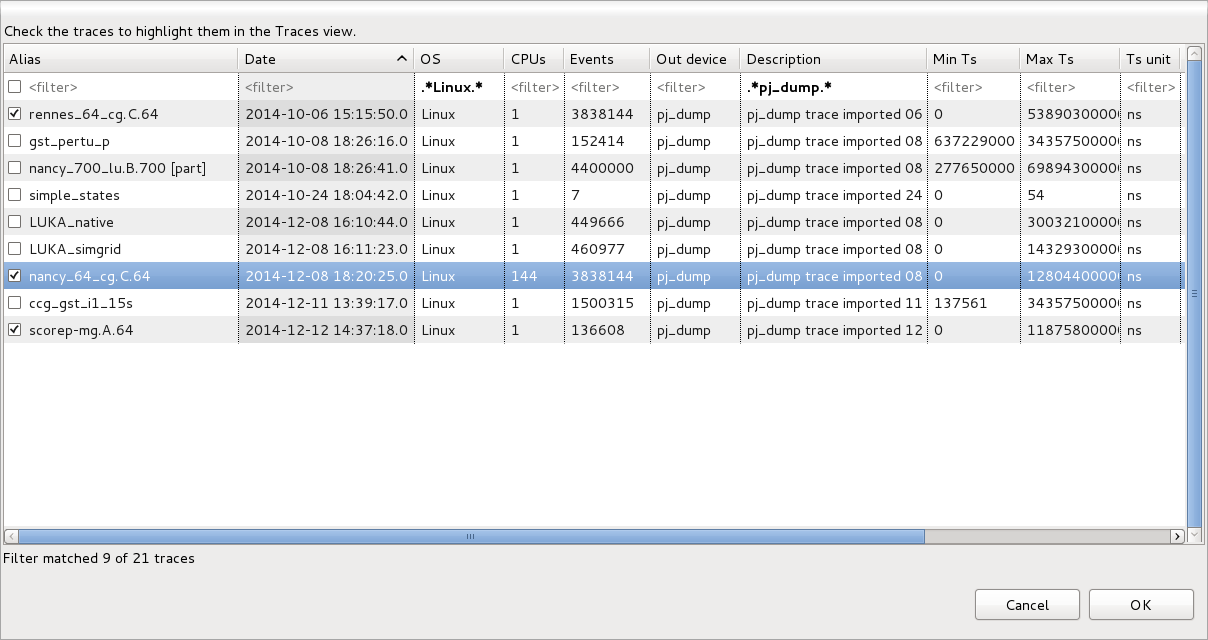
\includegraphics[width=0.9\textwidth]{images/trace_table_filter.png}
  \caption{Trace Filter Dialog}
  \label{fig:trace_filter_dialog}
\end{figure}

This dialog displays a table containing all the traces imported in the system. Each column of this table corresponds to a particular trace metadata. Clicking on the header of each column, it is possible to sort the table rows according to the column content. The first row of the table has editable fields, allowing for filtering on the corresponding column content. Filtering can be done using regular expression. At the bottom of the table, the number of traces matched by the filter, over the totality of traces, is displayed. In the example shown in Figure~\ref{fig:trace_filter_dialog}, we filtered all the traces produced on ``Linux'', containing the string ``pj\_dump'' in the description.

The first column of each row has a checkbox, allowing to select/deselect the corresponding trace. The checkbox in the first row (filter row) select/deselect all shown traces.
When pressing \emph{OK}, all selected traces are highlighted (shown in bold) in the trace browser (Figure~\ref{fig:highlight}). This allows the analyst to immediately spot interesting traces in the browser.

\begin{figure}[h!]
  \centering
    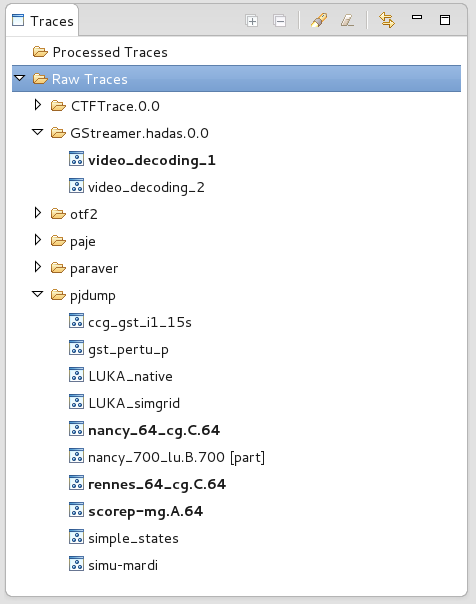
\includegraphics[width=0.5\textwidth]{images/trace_browser_highlight.png}
  \caption{Highlighted traces in Traces view}
  \label{fig:highlight}
\end{figure}

%------------------------------------------------------------------
\subsection{Trace Metadata Viewer/Editor}
\label{subsec:metadata}

\begin{figure}[h!]
  \centering
    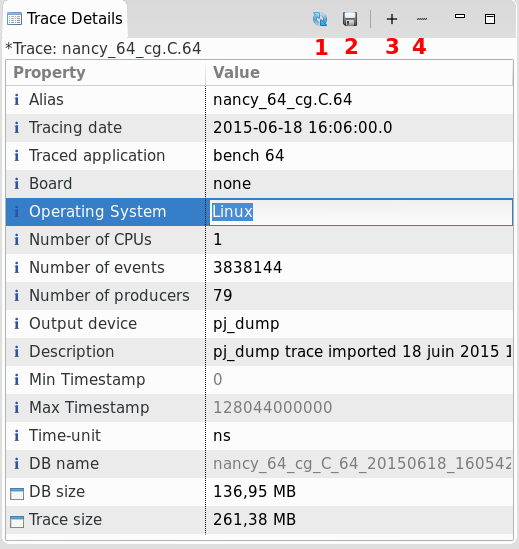
\includegraphics[width=0.5\textwidth]{images/metadata_editing.png}
  \caption{Trace Details view}
  \label{fig:metadata_editing}
\end{figure}

The \emph{Trace Details} view (Figure~\ref{fig:metadata_editing}) is the Framesoc perspective trace metadata viewer and editor.
When a trace is selected in the \emph{Traces} view, the trace metadata are displayed in a table viewer containing two columns: the property name and the property value.
If more than one trace is selected in the \emph{Traces} view, only the properties having the same name and the same values are shown.
The different properties are grouped in two different categories: predefined properties (displayed first) and custom properties (displayed last). 
Those categories are identified by two different icons.
The \emph{Value} column is normally editable, with the exception of some properties that are read only.
In order to edit an editable property value, the user simply has to click the value and modify it (as shown in Figure~\ref{fig:metadata_editing} for the \emph{OS} property).
When one or more values have been modified, a star (\emph{*}) is displayed before the trace alias, on top of the table, and the two view toolbar buttons \num{1} and \num{2} are enabled. 
The \emph{Reset changes} button (\num{1}) restores all non-saved edited properties to their previous value.
The \emph{Save changes} button (\num{2}) stores the changes.
%% TODO the notification must be done for any metadata change!!! cfr. issue #106
If the \emph{Alias} predefined property of a trace is persistently modified, other views are notified in order to take the necessary actions (e.g., update their label for the trace).

The other two buttons in the toolbar (\num{3} and \num{4}) allows for adding and removing custom trace metadata to the currently selected traces. Pressing the button indicated with \num{3} in Figure~\ref{fig:metadata_editing} will display a dialog to add a new property (Figure~\ref{fig:new_metadata}).

\begin{figure}[h!]
  \centering
    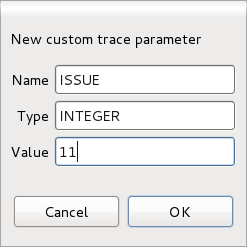
\includegraphics[width=0.3\textwidth]{images/new_metadata.png}
  \caption{Dialog to add a new custom property as trace metadata}
  \label{fig:new_metadata}
\end{figure}

In the example shown in Figure~\ref{fig:new_metadata}, after pressing \emph{OK}, a new trace property \texttt{ISSUE} of type \texttt{INTEGER} and value \texttt{11} is added to the selected trace. The trace metadata will therefore look as shown in Figure~\ref{fig:metadata_remove}. In this figure it is possible to see that, when selecting a custom property, the \emph{Remove property} button (indicated as \num{4} in Figure~\ref{fig:metadata_editing}, where it is disabled) is enabled and can be used to remove the selected custom property.

\begin{figure}[h!]
  \centering
    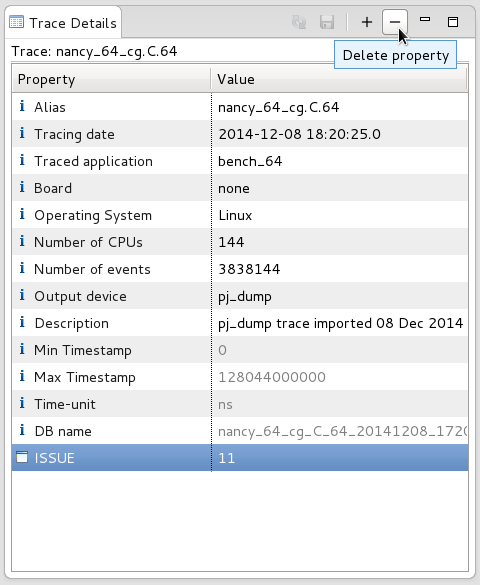
\includegraphics[width=0.5\textwidth]{images/metadata_remove.png}
  \caption{Trace Details view after adding a custom property (ISSUE)}
  \label{fig:metadata_remove}
\end{figure}

Note that if more than one trace is selected in the \emph{Traces} view, it is still possible to edit, add or remove properties.

%=====================================================================
\section{Analysis Views}
\label{sec:analysis}
%=====================================================================

%------------------------------------------------------------------
\subsection{General principles}
\label{subsec:principles}

Before describing in detail the different Framesoc analysis views, we present here some general principles that hold for all such views.

\paragraph{Data management} 

All Framesoc analysis views try to maximize the interactivity and responsiveness of the system by pipelining data loading and visualization. This allows the user to start working with data (or at least visualize it), while the loading job is ongoing. For example, the Gantt chart allows for zooming in/out or panning the visualized part of the trace, while trace events are being loaded. 

The user has full control on the loading job, and can stop it when she wants. In this case, the data loaded so far are still available for analysis. To cancel a loading job, the user uses the \emph{Progress} view (see for example Figure~\ref{fig:progress} for the \emph{Progress} view showing the Gantt loading process.).

\begin{figure}[h!]
  \centering
    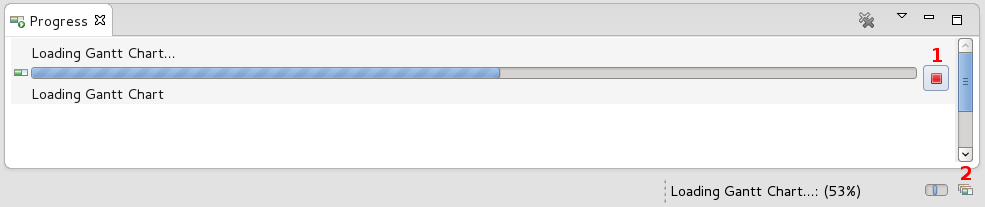
\includegraphics[width=0.9\textwidth]{images/loading.png}
  \caption{Progress view enabling to cancel a loading job}
  \label{fig:progress}
\end{figure}

The button indicated as \num{1} requests for stopping the job. The \emph{Progress} view is not shown by default in the Framesoc perspective. To access this view, the user has to click on the button indicated as \num{2}, which is always visible in Eclipse when a job is in progress.

\paragraph{Time management} Each Framesoc view is capable to load and display trace data related to whatever trace time interval: it is not compulsory to load in memory the entire trace to show only a given portion of it; it is possible, on the contrary, to load only a specific sub-interval. For example, the user has the flexibility to load only a specific time window of interest in the Gantt chart, avoiding charging into memory portions of the trace that are not interesting for the analysis.

The user controls the portion of the trace actually loaded into memory and displayed in the analysis view using a time management bar, located at the bottom of each Framesoc analysis view (Figure~\ref{fig:timebar}).

\begin{figure}[h!]
  \centering
    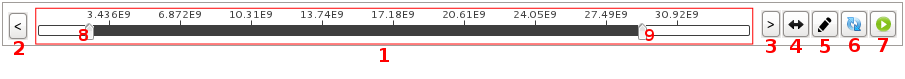
\includegraphics[width=0.9\textwidth]{images/time_bar.png}
  \caption{Time management bar present in all Framesoc analysis view}
  \label{fig:timebar}
\end{figure}

This bar contains a double range time slider (\num{1}) representing the whole trace duration, surrounded by two arrow buttons (\num{2} and \num{3}), and followed by four more buttons on the right (\num{4}, \num{5}, \num{6} and \num{7}).
The two knobs of the double range slider (\num{8} and \num{9}) identify the portion of the trace (colored in black) actually loaded in the table.
Using this kind of representation, the user always keeps a global visibility on the whole trace, while loading only the information he is interested in.
In order to change the time window loaded in the view, the user has to change the width of the black bar using the knobs \num{8} and \num{9}.
However, in order to avoid spurious and useless data transfers (from disk to memory), the new time interval is actually loaded only when the user presses the button indicated as \num{7}.
The button indicated as \num{6} resynchronizes the time bar with the time window actually loaded in the table, if they differ (i.e., the user modified the interval in the timebar without triggering a load with button \num{7}).
In order to modify the time window visualized in the double range slider the user has several possibilities. 
\begin{itemize}
 \item \emph{Graphical selection}: it is the most intuitive way and it involves using the two knobs \num{8} and \num{9}, in order to graphically set the two bounds of the time interval.
 \item \emph{Time window navigation}: this possibility involves using the two arrow buttons \num{2} and \num{3}, to select a time window that has the same size that the currently visualized one, but is located immediately before or immediately after the current one.
 \item \emph{Manual selection}: by pressing the button indicated as \num{5}, the user accesses a dialog (Figure~\ref{fig:window_dialog}) where it is possible to explicitly put the exact values of the time interval start and end timestamps. 
 This dialog enables also a manual definition of the size of the time window to be used when performing the \emph{time window navigation} described above.
 \item \emph{Select all}: using the button indicated as \num{4}, the user easily selects the whole trace duration.
\end{itemize}

\begin{figure}[h!]
  \centering
    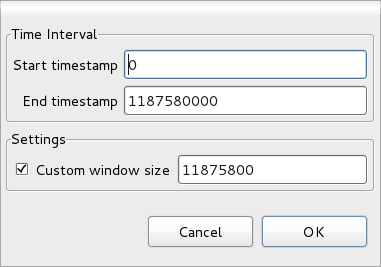
\includegraphics[width=0.35\textwidth]{images/window_dialog.png}
  \caption{Time window dialog}
  \label{fig:window_dialog}
\end{figure}

Regarding timestamps representation in Framesoc, if no time unit is indicated beside a displayed timestamp, 
by default the time unit used is the one shown in the \emph{Trace Details} (Section~\ref{subsec:metadata}) view for that trace (\texttt{Time-Unit} metadata). 
This applies to the time management bar described above, as well as to any other Framesoc GUI place.


\paragraph{Event producer and event type filter}
The pie chart, the histogram and the Gantt chart views all have filter options in order to give the users more control over their analysis. These filters allow to select the event producers and the event types used when computing the statistics. These filters can be accessed through the buttons in Figure \ref{fig:filterButtons} that are in the top right corner of the views. Clicking on one of these buttons will open a new dialog. 

\begin{figure}[h!]
	\centering
		
\includegraphics[width=0.1\textwidth]{images/filterButtons.png}
	\caption{Filter buttons}
	\label{fig:filterButtons}
\end{figure}

\begin{figure}[h!]
 \centering
 \begin{subfigure}[c]{0.46\textwidth}
    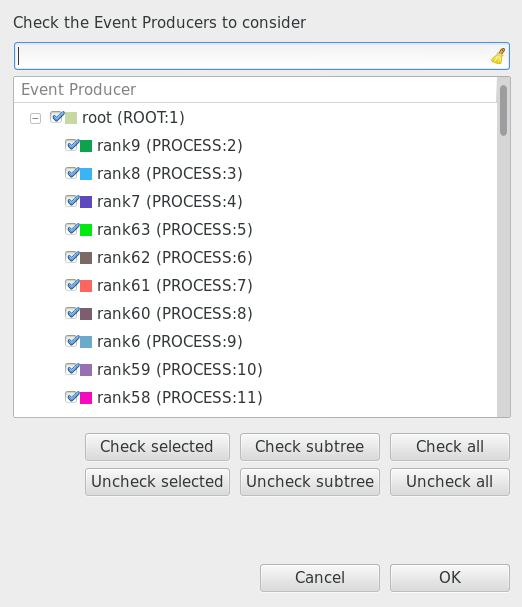
\includegraphics[width=1.0\textwidth]{images/ep_filter.png}
    \caption{Event producer filter dialog}
    \label{fig:eprod_dialog}
 \end{subfigure}%
 \hspace{30pt}
 \begin{subfigure}[c]{0.46\textwidth}
    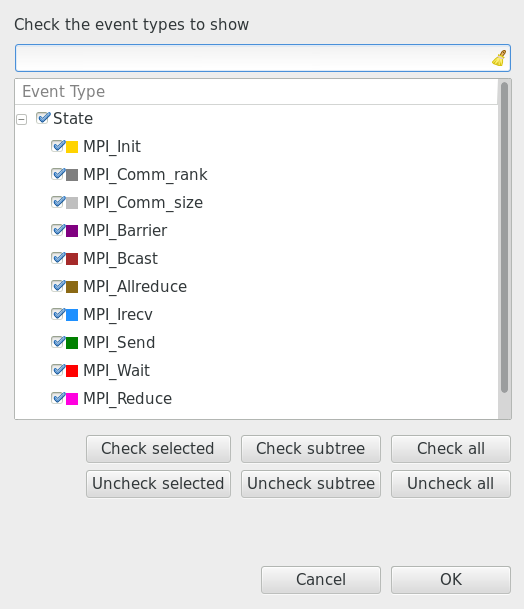
\includegraphics[width=1.0\textwidth]{images/event_filter.png}
    \caption{Event type filter dialog}
    \label{fig:etype_dialog}         
 \end{subfigure}
 \caption{Framesoc filters}
 \label{fig:dbms_configuration}       
\end{figure}

For the event producer filter dialog, shown in Figure \ref{fig:eprod_dialog}, all the event producers are displayed as a hierarchy tree, where each node and leaf is a checkbox that allow to select the event producer. At the bottom of the window, several buttons are available that allow to perform select operations. These buttons are:
\begin{itemize}
	\item \emph{Check/Uncheck Selected:} select/unselect the selected producer.
	\item \emph{Check/Uncheck Subtree:} select/unselect the selected producer and all its children in the hierarchy.
	\item \emph{Check/Uncheck All:} select/unselect all the event producers. 
\end{itemize}
At the top of the hierarchy tree, an editable text field can be used to search among the event producers.

The event type filter dialog, illustrated in Figure \ref{fig:etype_dialog}, displayed all the event types present in the current trace. The event types are displayed as a hierarchy tree where they are grouped by their category (i.e. punctual event, state, link or variable). The dialog is similar to the event producer one, described in the previous paragraph, including the text field to search among the event types and the buttons to perform the select operations.

Note that as opposed to the time management bar, where in order to perform the filtering on time the user has to press a button, these filters are applied and the view updated immediately after the user has pressed the \emph{OK} button in the dialog.

\paragraph{View communication} Using the Framesoc Bus (described in the RT-447~\cite{pagano:hal-00977887}), Framesoc views can communicate with each other. This mechanism is mostly used to synchronize the different views on time intervals, and to propagate to all the views changes in colors (see Subsection~\ref{subsec:colors}) or trace metadata (see Subsection~\ref{subsec:metadata}).
Regarding time interval synchronization, in the toolbar of each Framesoc analysis view, there are some \emph{Show in...} buttons, allowing the user to pass from one view to another, still keeping the same trace and the same time interval. Figure~\ref{fig:show_in} shows all the possible \emph{Show in...} buttons. 

\begin{figure}[h!]
  \centering
    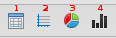
\includegraphics[width=0.2\textwidth]{images/show_in_icons.png}
  \caption{\emph{Show in...} toolbar buttons}
  \label{fig:show_in}
\end{figure}

Button \num{1} switches to the event table view (see Subsection~\ref{subsec:table}). Button \num{2} switches to the Gantt chart view (see Subsection~\ref{subsec:gantt}). Button \num{3} switches to the statistics pie chart view; in this case, a dialog is shown to the user in order to select one of the possible statistics operators (see Subsection~\ref{subsec:pie}). Button \num{4} switches to the event density chart view (Subsection~\ref{subsec:histogram}).

Of course, a view toolbar does not have a button redirecting to the view itself, so only three out of four possible \emph{Show in...} buttons are displayed in each view toolbar.

\paragraph{Group of view}
If the \emph{Allow view replication} option in the preferences is enabled (see Subsubsection \ref{subsec:gui}), it is possible to open several views on the same trace. This is done by right-clicking on a trace in the Trace browser and, if a view of an analysis tool is already opened with this trace, then the \emph{Show another...} menu item appears. Clicking on this option will open a new view with the selected trace and also creates a new \emph{group of view}. A group defines a family of different types of views (i.e., Gantt, Pie, etc.) for a given trace. Each instance of a view of an analysis tool belongs to a different group. Thus, if the user performs a switch to another view, if the group of view does not yet contain an instance of this view and if the maximum number instance of a view set in the option has not been reached, a new instance of the demanded view will be created. If a view already exists within the group, then this view is put forward and it is synchronized on time (as described in the previous paragraph).  When there are at least two groups of view for the same trace, the name of the trace in the views is preceded by a number identifying the group to which it belongs.

%------------------------------------------------------------------
\subsection{Statistics Pie Chart}
\label{subsec:pie}

\begin{figure}[h!]
  \centering
    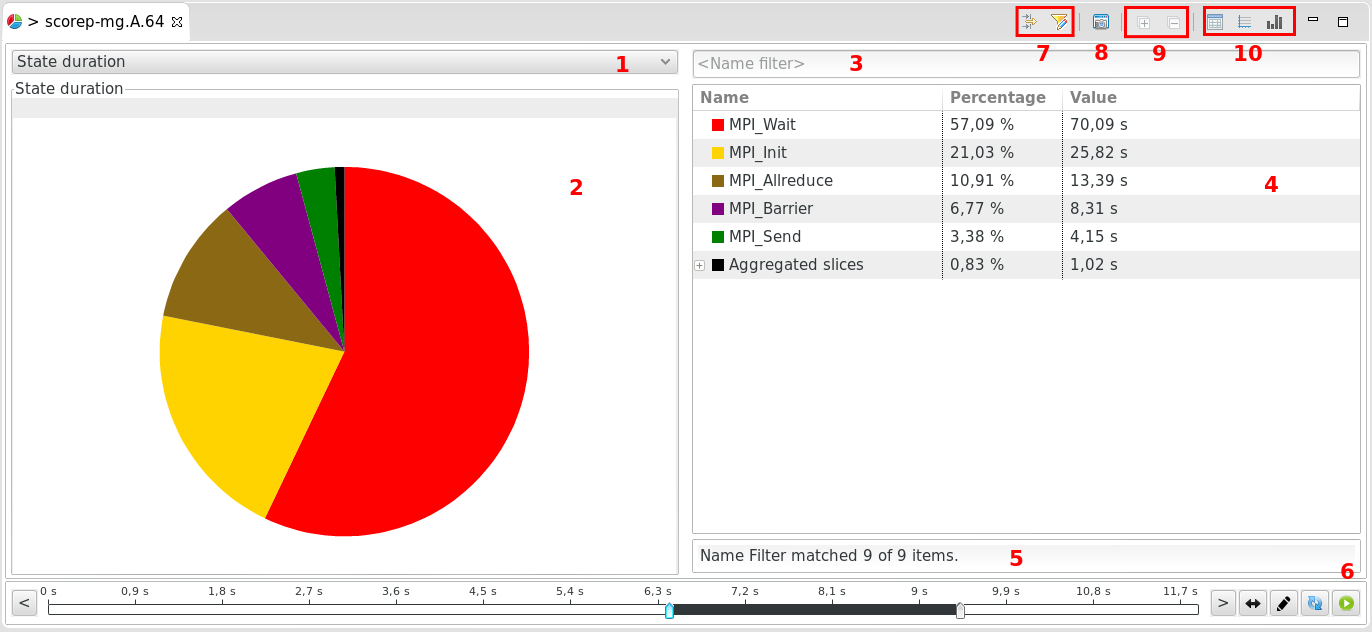
\includegraphics[width=1.0\textwidth]{images/pie.png}
  \caption{Statistics Pie Chart view}
  \label{fig:pie_chart}
\end{figure}

The \emph{Statistics Pie Chart} view (Figure~\ref{fig:pie_chart}) is a Framesoc analysis view presenting several metrics in the form of a pie chart.
The view is composed of two parts.
On the left, there are the metric selector (\num{1}) and the actual pie chart (\num{2}).
On the right, a table viewer (\num{4}) displays the same information as the pie chart. 
The table has three columns: the pie-slice name, the percentage value and the actual value. 
The name column cells contain a small square icon, filled with the color corresponding to the slice.
Each column header, when clicked, triggers the sorting of the rows according to the values in the corresponding column.
The content of this table viewer can be filtered by name using the text field on top of it (\num{3}). 
The number of items matched by the filter, over the totality of items, is shown in the status bar under the table viewer (\num{5}).
At the bottom of the view, there is the time management bar described in Subsection~\ref{subsec:principles}.

For the time being, four metrics are available: 
\begin{itemize}
 \item Event Producer instances: each slice represents the number of events having a given event producer.
 \item Event Type instances: each slice represents the number of events having a given event type.
 \item Link duration: each slice represents the duration of a given type of links.
 \item State duration: each slice represents the duration of a given type of state.
\end{itemize}
Note that each metric is computed considering only the selected time interval.

From Figure~\ref{fig:pie_chart} it is possible to note that there can be a special slice in the pie: the \emph{Aggregated} slice.
This slice aggregates all the slices whose value is smaller than a given threshold, being therefore difficult or impossible to see.
This threshold has been empirically set to $1\%$, taking into account user ergonomics and screen limitations.
In the table on the right, the \emph{Aggregated} slice corresponds to a folder entry, whose sub-entries are the actual slices.
All the detailed information is thus kept and made available in the tabular representation.

By right clicking on one or more of the table elements, a context menu is shown.
The commands available in this menu vary according to the elements selected.
If the \emph{Aggregated} slice row is selected, no menu is shown.
In any other case, the menu can contain one or more of the following commands:
\begin{itemize}
 \item \emph{Exclude Item from statistics / Exclude items from statistics}: shown if only leaf items are selected. This command excludes the selected leaf items from statistics computation. If there is at least one excluded item, the number of excluded items is shown in the status bar (\num{5}).
 \item \emph{Merge Items}: shown only if two or more leaf items are selected. This command merges the items in a new folder item. The name and the color of the new folder item are chosen by the user with the dialog shown in Figure~\ref{fig:merge_dialog}.
    \begin{figure}[h!]
      \centering
	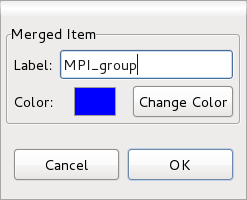
\includegraphics[width=.25\textwidth]{images/dialog_merge.png}
      \caption{Merge Items Dialog}
      \label{fig:merge_dialog}
    \end{figure} 
 \item \emph{Unmerge Items}: shown if one or more folder items are selected. This command unmerges the items contained in the folder item.
 \item \emph{Unmerge All Items}: shown if at least one folder item, created by merging two or more leaf items, exists. This command unmerges all the merged items. 
 \item \emph{Restore Excluded Items}: shown if at least one leaf item has been excluded from statistics computation. This command restores all previously excluded items into statistics computation.
\end{itemize}

Note that when a \emph{Statistics Pie Chart} view is opened for a given trace using the context menu in the trace browser, no pie chart is actually displayed, since the user has to select the metric of interest first, then press the load button (\num{6}) in the time management bar.

The view toolbar contains the \emph{Show in...} buttons (\num{9}), the filter button (\num{7}) and a couple of buttons to expand/collapse the folder items in the table (\num{8}).

%------------------------------------------------------------------
\subsection{Event Density Chart}
\label{subsec:histogram}

\begin{figure}[h!]
  \centering
    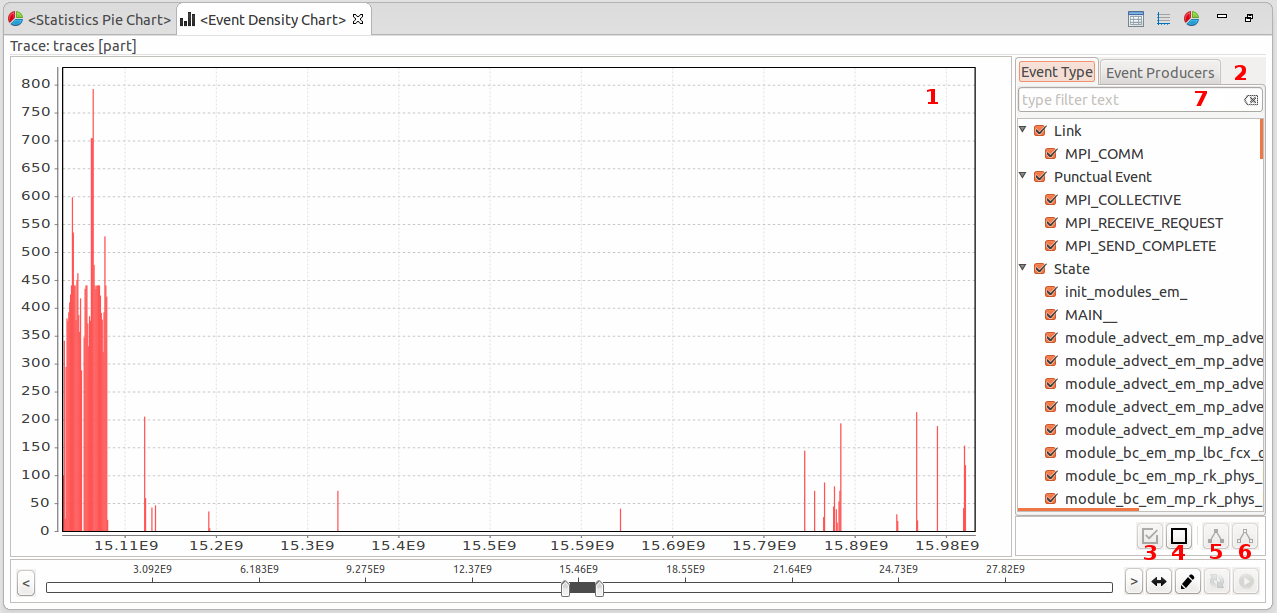
\includegraphics[width=1.0\textwidth]{images/histogram.png}
  \caption{Event Density Chart view}
  \label{fig:histogram}
\end{figure}

The \emph{Event Density Chart} view (Figure~\ref{fig:histogram}) is a Framesoc analysis view displaying the event density over time in the form of a histogram.

In the histogram (\num{1}), the $x$ axis represents the time, while the $y$ axis represents the number of events.
The histogram number of bins is fixed and has been chosen taking into account the number of pixels actually present on a screen, to ensure a clear visualization. 
The user can zoom in and out on portions of the chart.
In particular, to zoom in on a portion of the chart, the user has to click at the start of the portion, drag the mouse going to the right up to the end of the portion, then release the click.
To zoom out completely, the user has to do the same as above, but dragging the mouse to the left this time.
When hovering the mouse on a bin, some information about the bin is displayed: the central timestamp and the number of events.

In top right corner, there is the event type and event producer filter buttons (\num{2}), and the view switching buttons (\num{3}). The features of these buttons are described in Subsection \ref{subsec:principles}.

At the bottom of the view, there is the time management bar described in Subsection~\ref{subsec:principles}.
The event density is computed considering only the events in the selected time interval, for the selected types and the selected producers.

%------------------------------------------------------------------
\subsection{Event Table View}
\label{subsec:table}

\begin{figure}[h!]
  \centering
    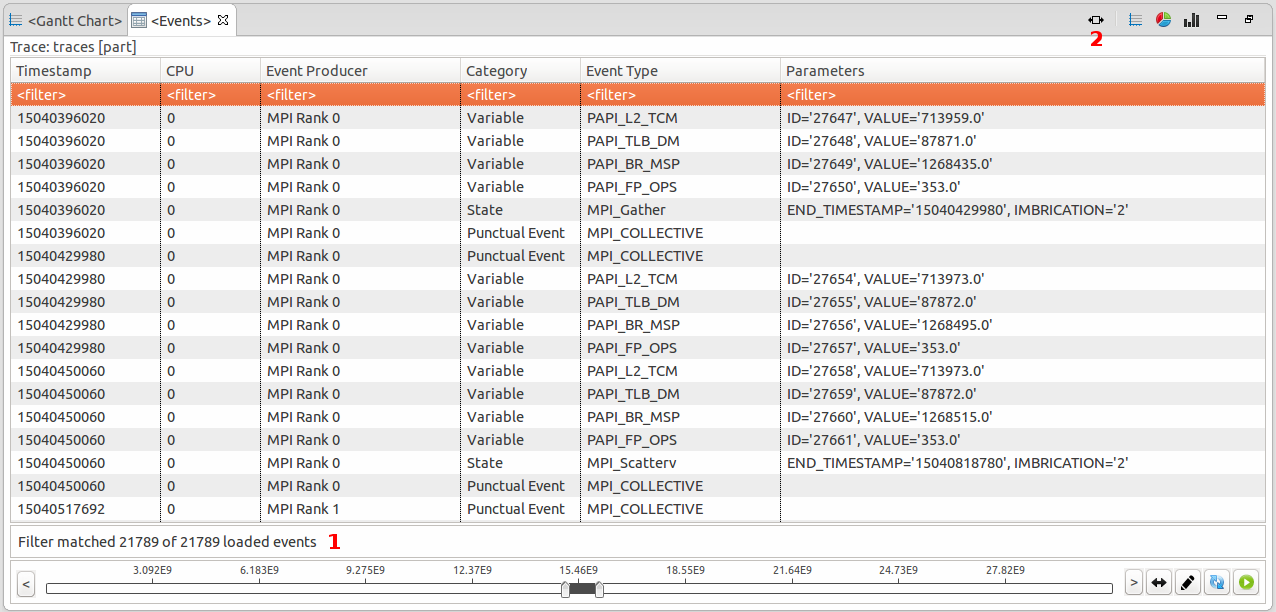
\includegraphics[width=1.0\textwidth]{images/table.png}
  \caption{Events view}
  \label{fig:table}
\end{figure}

The \emph{Events} view (Figure~\ref{fig:table}) is a Framesoc analysis view showing a tabular representation of trace events.
The main element of this view is a table viewer, displaying a distinct row for each event of the trace.
This table has the following columns:
\begin{itemize}
 \item Timestamp: the event timestamp.
 \item CPU: the number of the CPU on which the event has been produced.
 \item Event Producer: the name of the entity producing the event.
 \item Category: the event category (State, Link, Punctual Event, Variable).
 \item Event Type: the event type name.
 \item Parameters: the list of the event custom parameters, with the format \texttt{NAME='VALUE'}.
\end{itemize}
The first row of the table contains an editable filter for each column. 
These filters accept regular expressions.
The number of events matched by the filter, over the totality of loaded events, is shown in the status bar under the table viewer (\num{1}).
Filtering takes place in a separate thread and can be stopped pressing \texttt{ESC}. 
All filters can be cleaned contextually pressing \texttt{DEL}.

At the bottom of the view, there is the time management bar described in Subsection~\ref{subsec:principles}.

Beside the three \emph{Show in...} buttons indicated as \num{3} (see Subsection~\ref{subsec:principles}), the view toolbar contains a button (\num{2}) that resizes column width to fit the actual content.

%------------------------------------------------------------------
\subsection{Gantt Chart View}
\label{subsec:gantt}

\begin{figure}[h!]
  \centering
    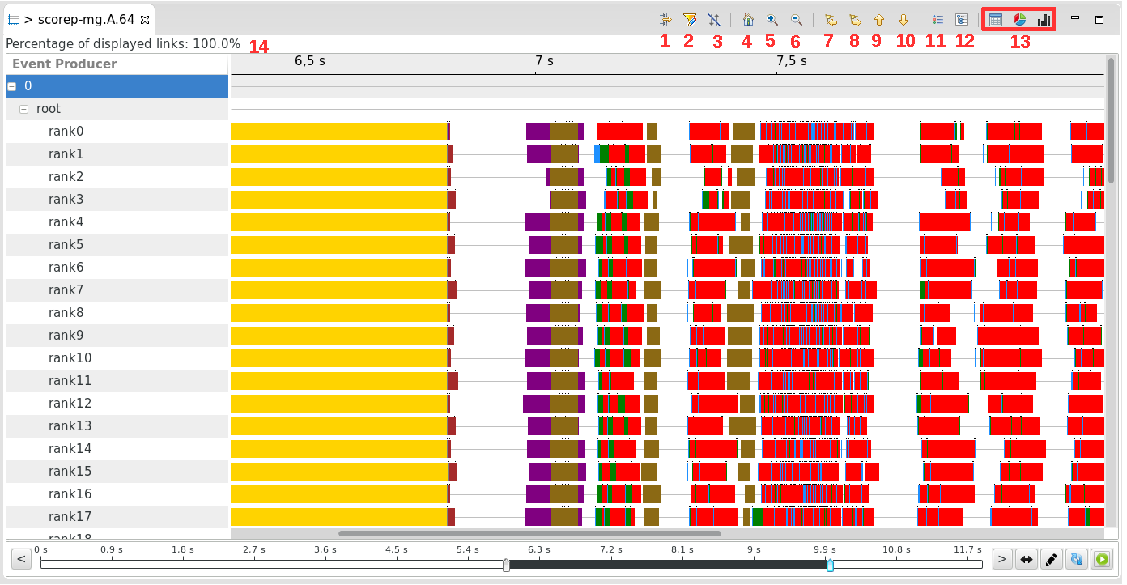
\includegraphics[width=1.0\textwidth]{images/gantt.pdf}
  \caption{Gantt Chart view}
  \label{fig:gantt}
\end{figure}

This view (Figure~\ref{fig:gantt}) shows a Gantt chart representation of trace events.
This kind of representation is pretty common in trace analysis frameworks (e.g., Lttng Eclipse Viewer~\cite{lttng_viewer}) and is classically used to visualize application behavior over time, thanks to its ability to represent causality relations~\cite{wilson_gantt_2003}.

The main element of this view is a Gantt viewer\footnote{The viewer is based on the one available in the Lttng Eclipse Viewer~\cite{lttng_viewer}}, which is composed of two parts.

On the left there is the hierarchy of event producers. 
Double clicking on a non-leaf node of the tree, the node is expanded/collapsed.
Right clicking on a node, a contextual menu is shown. 
For leaf nodes, the menu allows the user to hide them.
For non-leaf nodes, the menu allows the user to hide them and their sons, or to expand/collapse them.

On the right there is the actual time chart, showing for each producer all the punctual events it generates (represented as simple vertical lines) and all the states it spends time in (represented as colored rectangles). 
If there are links in the trace (e.g., communications), they are represented as oriented arrows.
The Gantt chart does not currently consider variables.
The colors used for the different entities depend on the event type.
When hovering the mouse on a given entity, a tooltip with detailed information is shown.
For each entity the tooltip contains specific information:
\begin{itemize}
 \item for a state: the producer, the type, the start/end timestamps and the duration.
 \item for a link: the source/target producers, the start/end timestamps and the duration.
 \item for a punctual event: the producer, the type and the timestamp.
\end{itemize}

Zooming in/out on a given point of the Gantt chart, is done putting the mouse on the point of interest, then moving the mouse wheel while pressing \texttt{CTRL}.
When zooming in/out the following functionalities can be triggered:
\begin{itemize}
 \item State aggregation: if there are not enough pixels to show all the states in a given time region, these states are aggregated and a black point is displayed above the point where the aggregation took place. 
 \item Link filtering: if there are not enough pixels to show all the links in a given time region, only the visible links are shown. 
 The percentage of shown links (computed over the total of links in the time region currently visible) is displayed above the Gantt chart (\num{14}).
 When there exist no links in the trace (in the time region currently visible) the percentage value is \texttt{100\%}. This state of this option is global, i.e. the future instances of the Gantt chart view will use the value of this option when it was last modified (e.g. if link display is turned off in the Gantt, all the next instances of the Gantt view will not display the links). 
\end{itemize}
These two functionalities keep the user aware of what is going on (information loss), thus reducing visual artifacts and possible analysis pitfalls.

The user can select a time region in the Gantt using the mouse (click on the start point, then drag and release on the end point). 
While selecting a given region, the same selection is applied to the time management bar present at the bottom of the view (see Subsection~\ref{subsec:principles}).
Similarly, changing the selection in the time management bar, changes the selection in the Gantt chart.
When a time region is selected, clicking on a given point of the Gantt chart removes the selection and restore the time management bar selection as it was before.

Beside the three \emph{Show in...} buttons indicated as \num{13} (see Subsection~\ref{subsec:principles}), the view toolbar contains the following buttons:
\begin{itemize}
	\item Button \num{1}: display a dialog where it is possible to select the event producers to display.
	\item Button \num{2}: display a dialog where it is possible to select the types to display.
	\item Button \num{3}: hide/display links.
	\item Button \num{4}: fit the zoom to the available screen space, to display all the loaded portion of the trace in the view.
    \item Button \num{5}: zoom in.
	\item Button \num{6}: zoom out.
  	\item Button \num{7}: select the previous event.
	\item Button \num{8}: select the next event.
	\item Button \num{9}: select the previous event producer line.
	\item Button \num{10}: select the next event producer line.
    \item Button \num{11}: display a dialog showing the color legend. 
	\item Button \num{12}: use the CPU drawer; the trace is reloaded using a different event producer hierarchy where CPUs are the roots.
\end{itemize}

%------------------------------------------------------------------
\section{Framesoc Menu and Toolbar}
\label{sec:menu}

When the Framesoc perspective is activated, the Framesoc menu (Figure~\ref{fig:menu}) and the corresponding toolbar (Figure~\ref{fig:toolbar}) are visible. 

In the menu, there are two items: the trace analysis menu and preferences.
The preferences allows the user to access database system configuration, GUI configuration, color management and tool management.
The trace analysis menu allows the user to launch importers, analysis tools and exporter tools.

In the toolbar, the different buttons are simply shortcuts for the above functionalities, where corresponding icons mean corresponding functionalities.
The added value of the toolbar is that, beside each of the three buttons used to launch the tools of the various category (import, analysis, export), there is a drop down menu containing the list of the tools of that category, useful to directly launch a tool.

In the following subsections, the functionalities accessible from the menu or the toolbar are explained in detail.

\begin{figure}[h!]
  \centering

    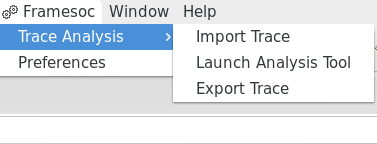
\includegraphics[width=0.4\textwidth]{images/menu.png}
  \caption{Framesoc Menu}
  \label{fig:menu}
\end{figure}

\begin{figure}[h!]
  \centering
    
\includegraphics[width=0.4\textwidth]{images/toolbar.png}
  \caption{Framesoc Toolbar}
  \label{fig:toolbar}
\end{figure}

\subsection{Preferences}
\label{subsec:pref}
The preferences dialog allows the user to configure various settings of Framesoc elements. There are four tabs in the preferences dialog: database, GUI, color management and tool management. The settings modified in this dialog are saved in the Framesoc configuration file (Appendix~\ref{app:conf}). 

\begin{figure}[h!]
	\centering
	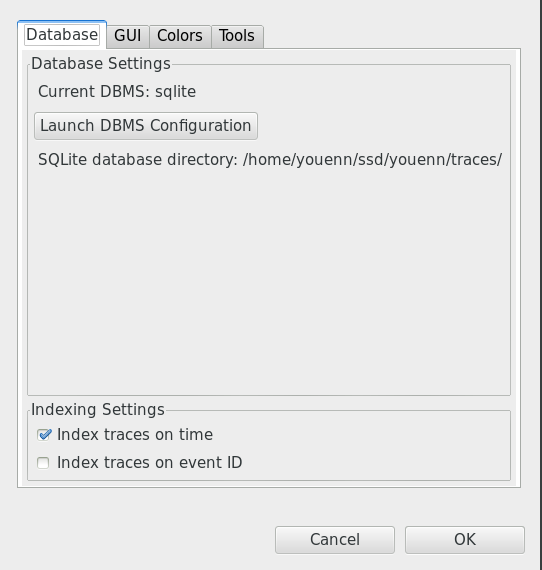
\includegraphics[width=.5\textwidth]{images/pref_db.png}
	\caption{Preferences dialog -- Database settings tab}
	\label{fig:pref_dialog_db}
\end{figure} 

\subsubsection{Database Settings}
The database settings tab, shown in Figure \ref{fig:pref_dialog_db}, is subdivided in two groups: database settings and indexing settings. 

The indexing settings allow the user to choose if the traces imported with any of the importers in Framesoc, will be indexed on time, on event ID or on both. 

The database settings group displays information about the currently used DBMS and its settings. If the current DBMS is SQLite, then the path to the current database is displayed. If the current DBMS is MySQL, then the user name and the URL of the database are shown. In order to modify the database settings, you have to click on the button \textit{Launch DBMS configuration}. This will open the DBMS configuration wizard described below.

\paragraph{DataBase Management System Configuration}
\label{subsec:init}

In the DataBase Management System (DBMS) configuration, the user accesses a configuration wizard, whose first page is shown in Figure~\ref{fig:dbms_selection}. 
This page allows the user to select the DBMS to be used for trace storage.
In fact, as described in the technical report RT-435~\cite{pagano:hal-00830008}, Framesoc can work with several DBMS.
At the moment, the support has been implemented for SQLite (recommended) and MySQL.

\begin{figure}[h!]
  \centering
    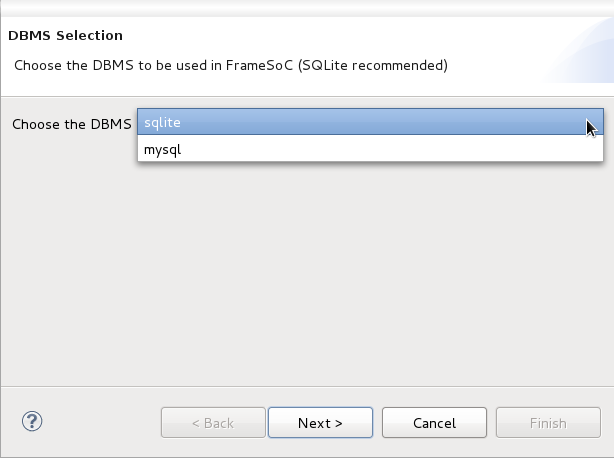
\includegraphics[width=0.5\textwidth]{images/dbms_selection.png}
  \caption{System Initialization: DBMS selection dialog}
  \label{fig:dbms_selection}
\end{figure}

Once the user has chosen the DBMS and pressed \emph{Next}, he comes to the DBMS configuration page (Figure~\ref{fig:dbms_configuration}), which is different for each DBMS.
If SQLite is selected (Figure~\ref{fig:dbms_configuration_sqlite}), the user simply has to enter the directory where he wants the database files to be kept.
Otherwise, if MySQL is chosen (Figure~\ref{fig:dbms_configuration_mysql}), the user has to specify some connection parameters (user-name, password, URL).

In both cases, after successfully pressing \emph{Finish}, the Framesoc storage subsystem is correctly configured. 
If a System DB already exists, it is reused, otherwise a new one is created.
This configuration is saved in the Framesoc configuration file (Appendix~\ref{app:conf}). 

\begin{figure}[h!]
 \centering
 \begin{subfigure}[c]{0.46\textwidth}
    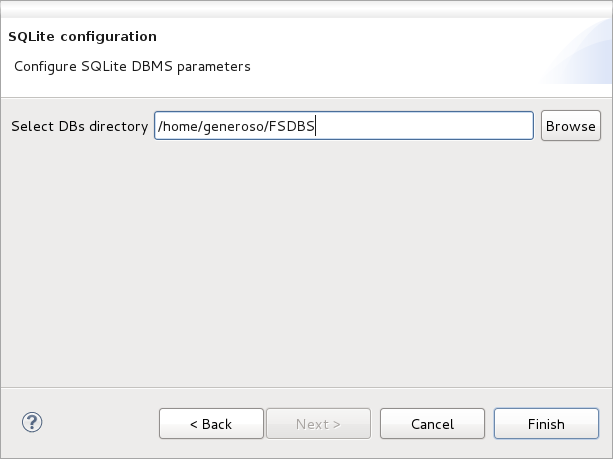
\includegraphics[width=1.0\textwidth]{images/dbms_configuration_sqlite.png}
    \caption{SQLite configuration dialog}
    \label{fig:dbms_configuration_sqlite}
 \end{subfigure}%
 \hspace{30pt}
 \begin{subfigure}[c]{0.46\textwidth}
    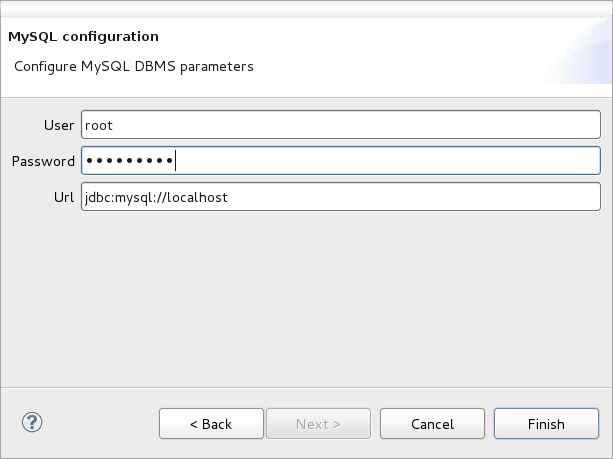
\includegraphics[width=1.0\textwidth]{images/dbms_configuration_mysql.png}
    \caption{MySQL configuration dialog}
    \label{fig:dbms_configuration_mysql}         
 \end{subfigure}
 \caption{System Initialization: DBMS configuration}
 \label{fig:dbms_configuration}       
\end{figure}

Note that after a modification of the database settings (at initialization or later), in the case of existing System DB, if there is a mismatch between the tools registered in this System DB and the tools actually present in the Framesoc Eclipse runtime\footnote{As described in the technical report RT-435~\cite{pagano:hal-00830008} the preferred way to add tools to Framesoc is to create an Eclipse plugin, extending a specific extension point defined by Framesoc. For this reason a tool is typically a plugin in the Framesoc Eclipse runtime.}, this is automatically fixed:
\begin{itemize}
 \item If a tool exists in the DB but not in the runtime, the tool is removed with its results (if any)\footnote{The user is asked for confirmation if the \texttt{ask\_for\_tool\_removal} variable is set to \texttt{true} in Framesoc configuration file (see Appendix~\ref{app:conf}).}.
 \item If a tool exists in the runtime but not in the DB, the tool is automatically registered.
\end{itemize}

The first time Framesoc is launched, the database configuration wizard is automatically launched in order to set up the initial configuration of the database.
Note also that at each Framesoc startup, the system automatically checks that the storage configuration is good. 
If it is not the case, the database configuration wizard is automatically launched.

A control for mismatch between runtime tools and System DB tools is also done at each startup, with the same policy as described above.

\subsubsection{GUI settings}
\label{subsec:gui}

\begin{figure}[h!]
	\centering
	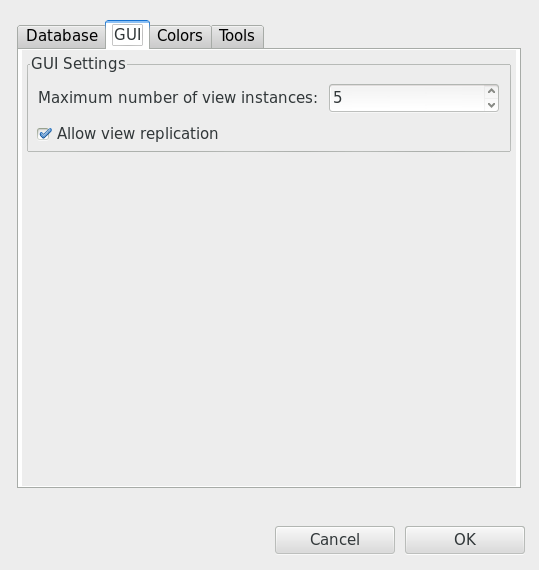
\includegraphics[width=.5\textwidth]{images/pref_gui.png}
	\caption{Preferences dialog -- GUI settings tab}
	\label{fig:pref_dialog_gui}
\end{figure}

In the GUI settings tab (Figure \ref{fig:pref_dialog_gui}), it is possible to configure two options that manage the views of the Framesoc analysis tools. The first option specifies the maximum number of instances of a view (e.g. the Gantt Chart) that can be opened simultaneously. The value can be set to -1, meaning that there will be no limit on the number of simultaneous instances. If the value is set to 0, then it is equivalent to a value of 1.

The second option is a checkbox that specifies if it is possible to open simultaneously several instances of the view on the same trace.

\subsubsection{Color Management}
\label{subsec:colors}

The color management tab (Figure~\ref{fig:color_type_list_MPI}) allows the user to modify the colors associated to event producers and event types in a centralized way for the whole workbench.
The combo box at the top (\num{1}) enables the selection of the entity (event producer or event type).
The list below enumerates all instances for a given entity, preceded by a small square icon filled with the instance color.
The editable text field on top of this list can be used as a filter on the list.
When an entity instance is selected, pressing the \emph{edit} button (\num{2}) gives access to the color edition dialog (Figure~\ref{fig:color_editing}).
Pressing \emph{OK} saves all the changes.
Pressing the \emph{reset} button (\num{3}) reverts unsaved changes for the current entity.
The color configuration for a given entity is physically stored in a configuration file located in the \texttt{configuration/fr.inria.soctrace.framesoc.ui} sub-folder of the Eclipse install directory.
For example, the relative path to Eclipse install directory of the event type color configuration file is:
\texttt{configuration/fr.inria.soctrace.framesoc.ui/event\_type\_colors}.

\begin{figure}[h!]
  \centering
  \begin{subfigure}[c]{0.46\textwidth}
    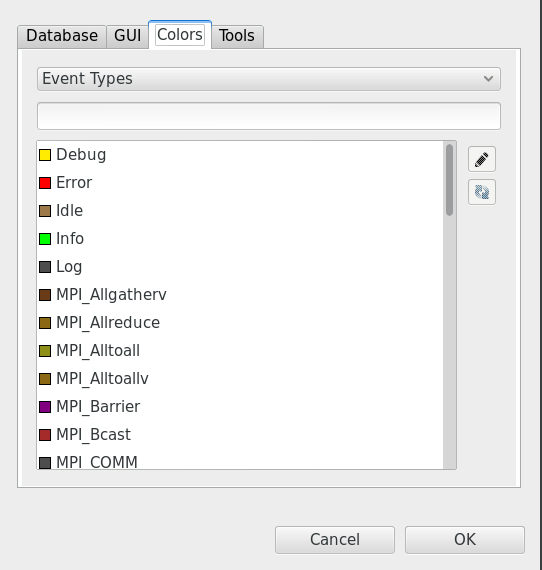
\includegraphics[width=1.0\textwidth]{images/pref_color.png}
    \caption{Color management tab}
    \label{fig:color_type_list_MPI}
  \end{subfigure}%
  \hspace{30pt}
  \begin{subfigure}[c]{0.46\textwidth}
    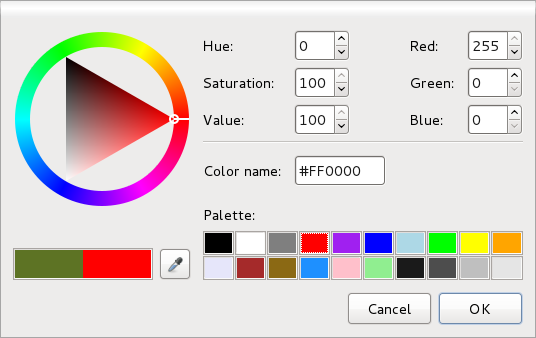
\includegraphics[width=1.0\textwidth]{images/color_editing.png}
    \caption{Color editing dialog}
    \label{fig:color_editing}       
  \end{subfigure}%
  \caption{Framesoc Color Management}
  \label{fig:colors}       
\end{figure}

Note that when \emph{OK} is pressed after changing some colors, the workbench modules are notified and the views may react by updating their colors in real-time.


\subsubsection{Tool Management}
\label{subsec:tools}

The tool management tab (Figure~\ref{fig:manage_tools}) simply displays the list of tools registered in the system, 
enabling the installation, modification and removal of external \emph{black-box} tools (tools that are not Eclipse plugins).

\begin{figure}[h!]
  \centering
    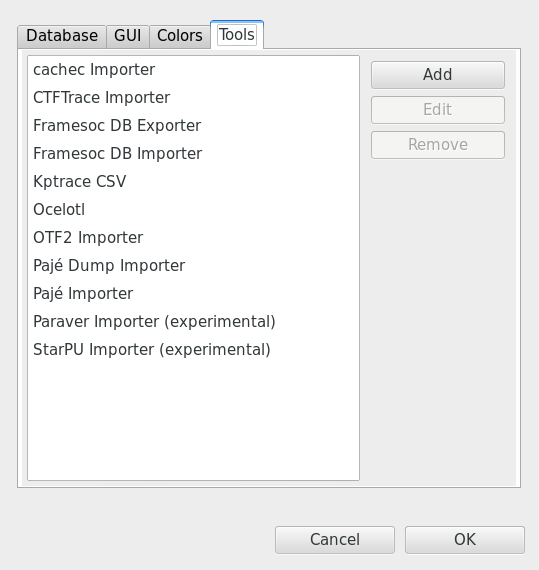
\includegraphics[width=0.5\textwidth]{images/pref_tool.png}
  \caption{Tool manager tab}
  \label{fig:manage_tools}
\end{figure}

\begin{figure}[h!]
  \centering
    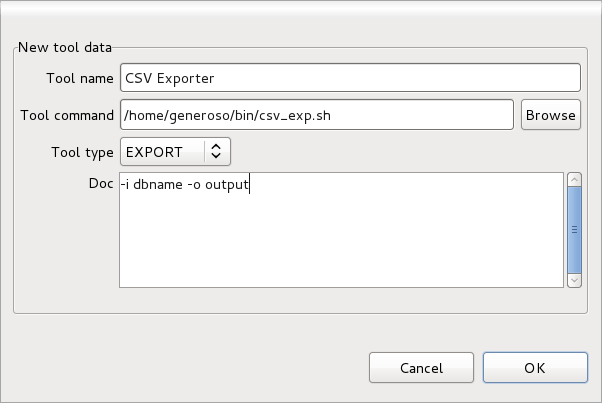
\includegraphics[width=0.5\textwidth]{images/blackbox.png}
  \caption{Black-box tool dialog}
  \label{fig:blackbox}
\end{figure}

Adding or modifying a \emph{black-box} tool requires the user to edit the different fields of the dialog displayed in Figure~\ref{fig:blackbox}.
In particular, the user has to pick a unique tool name, specify the launch command, select the tool type (import, analysis, export) and write the launch documentation.

Note that the use of external \emph{black-box} tools is discouraged, since most of the functionalities available using Eclipse plugins are not available.

Note also that plugin tools cannot be added, edited or removed via the manage tool dialog, since they are managed as standard Eclipse plugins.
Plugin tools are installed and removed using the normal Eclipse procedure (\textbf{Help $>$ Install New Software...} menu). 


\subsection{Trace Import}
\label{subsec:import}

The trace import dialog (Figure~\ref{fig:import_dialog}) allows the user to import new traces into the system, by using one of the registered importer tools.
The combo box on top of the dialog enables the selection of the importer.
The controls displayed below the combo box change according to the selected importer.
These controls allow the user to configure the importer and pass the needed input.
For example, in Figure~\ref{fig:import_dialog} we can see that the \emph{Pajé Dump Importer} has a checkbox to enable double precision and a text field for passing trace files.
Any tool specific message, triggered by a change in the input for example, is displayed in the text field at the bottom of the dialog (\emph{Tool Message} group).
The \emph{OK} button becomes active only if the input specified is considered valid by the tool. 
Pressing \emph{OK}, the import process is launched with the provided input.
At the end of this process, the trace browser view is automatically updated with the new trace information.

\begin{figure}[h!]
  \centering
    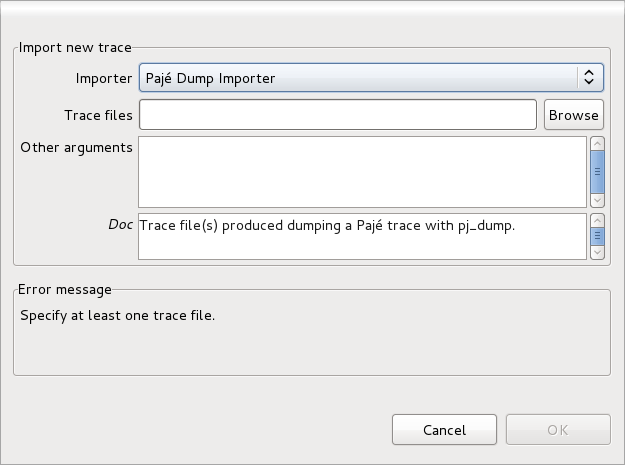
\includegraphics[width=0.5\textwidth]{images/import_dialog.png}
  \caption{Import trace dialog}
  \label{fig:import_dialog}
\end{figure}

\subsection{Launch Analysis Tool}
\label{subsec:analysis}

The launch analysis tool dialog (Figure~\ref{fig:analysis_dialog}) allows the user to launch one of the analysis tools registered in the system.
This dialog has the same structure than the Import Trace dialog (see Subsection~\ref{subsec:import}). 
Pressing \emph{OK}, the selected analysis tool is launched with the provided input. 

\begin{figure}[h!]
  \centering
    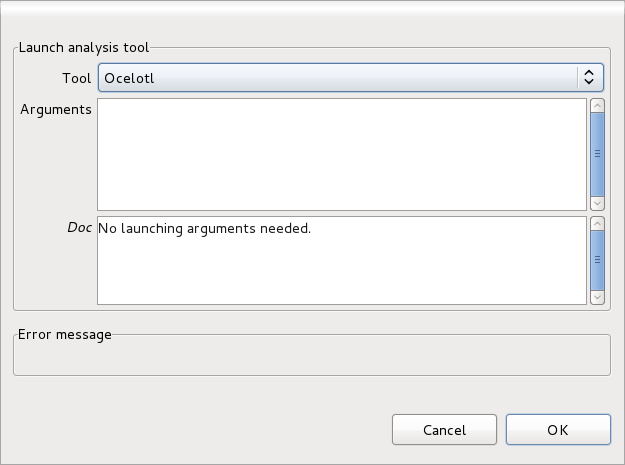
\includegraphics[width=0.5\textwidth]{images/analysis_dialog.png}
  \caption{Launch analysis dialog}
  \label{fig:analysis_dialog}
\end{figure}

\subsection{Trace Export }
\label{subsec:export}

The launch export tool dialog (Figure~\ref{fig:analysis_dialog}) allows the user to launch one of the export tools registered in the system.
This dialog has the same structure than the Import Trace dialog (see Subsection~\ref{subsec:import}). 
Pressing \emph{OK}, the selected export tool is launched with the provided input. 

\begin{figure}[h!]
  \centering
    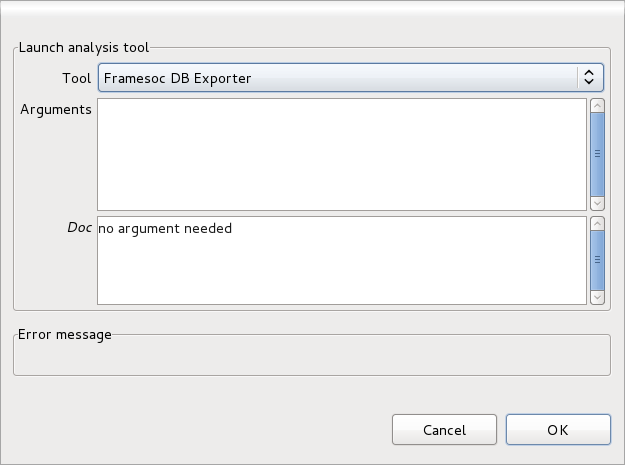
\includegraphics[width=0.5\textwidth]{images/export_dialog.png}
  \caption{Export trace dialog}
  \label{fig:export_dialog}
\end{figure}

\newpage

\appendix

%%=====================================================================
\section{Framesoc Configuration File}
\label{app:conf}
%%=====================================================================

The Framesoc configuration file is located within the Eclipse installation directory.
Its relative path to this directory is:  \texttt{./configuration/fr.inria.soctrace.lib.utils/soctrace.conf}. Note that if the Eclipse directory does not have the write permission, the configuration file will be created in the user home directory with the same relative path as above. Please note that it is not recommended to modify this file manually, but preferably by using the \textit{Preferences} dialog described in Subsection \ref{subsec:pref}. 

This file is automatically generated and mostly configurable using the GUI. 
It contains the following parameters:
\begin{description}
 \item[soctrace\_dbms]: DBMS used by Framesoc. The accepted values are: sqlite, mysql.
 \item[mysql\_db\_user]: MySQL database user name.
 \item[mysql\_db\_password]: MySQL database password.
 \item[mysql\_base\_db\_jdbc\_url]: MySQL database connection URL.
 \item[sqlite\_db\_directory]: Directory containing the SQLite database files.
 \item[soctrace\_db\_name]: Name of the Framesoc System DB.
 \item[max\_view\_instances]: Maximum number of instances for a given type of analysis views.
 \item[trace\_db\_indexing]: Boolean stating if automatic time indexing is done at trace import.
 \item[ask\_for\_tool\_removal]: Boolean stating if user confirmation must be asked when removing a tool and its results.
\end{description}

%% bibliography
\newpage
\renewcommand{\refname}{References}
\bibliography{framesoc_biblio}{}
\bibliographystyle{unsrt}
%%

%%=====================================================================
%%=====================================================================
\end{sloppypar} 
\end{document}
%%=====================================================================
%%=====================================================================

\endinput
%%
%% End of file.
